% questions.tex —— 1977 年·天津卷 · 题目内容片段（无答案）
% 由 tools/generate_projects.py 依来源总账自 1977/1977_数学真题_天津_试题.md 生成，勿手改（改源 MD 后重跑）


\gkpart{数学试卷（天津卷）}

\begin{gktip}
\textbf{来源说明}：本题面依据固定源 PDF《1977 天津卷数学试卷》第 1 页逐题转录。源文件为 A3 单页扫描，原卷未附答案页；配套答案与解析为本库编者独立推导，\textbf{非官方标准答案}。原卷第 6、7 题位于“附加题”栏，不计入正式题量。
\end{gktip}

\par\medskip

\begin{question}
\gkti{1}

（1） 在什么条件下，$\dfrac{y}{2x}$

① 是正数；

② 是负数；

③ 等于零；

④ 没有意义？

（2） 比较下列各组数的大小，并说明理由。

① $\cos31^\circ$ 与 $\cos30^\circ$。

② $\log_2 1$ 与 $\log_2\dfrac14$。

（3） 求值：

① $\tan\left(5\arcsin\dfrac{\sqrt3}{2}\right)$。

② $(-2)^0\times(0.01)^{\frac12}$。

\Needspace{5\baselineskip}
（4） 计算：

\nopagebreak[4]
\[
\lg12.5-\lg\frac58+\lg\sin30^\circ.
\]

\Needspace{5\baselineskip}
（5） 解方程：

\nopagebreak[4]
\[
\frac{4x}{x^2-4}-\frac2{x-2}=1-\frac1{x+2}.
\]

\Needspace{0.4\textheight}
\end{question}
\begin{question}
\gkti{2}

（1） 某工厂准备在仓库的一侧建立一个矩形储料场（如图），现有 $50$ 米长的铁丝网，如果用它来围成这个储料场，那么长和宽各是多少时，这个储料场的面积最大？并求出这个最大的面积。
\nopagebreak[4]
\begin{center}% 1977 年天津卷第 2(1) 题：仓库一侧的矩形储料场
\begin{tikzpicture}[scale=0.78,>=stealth]
  \draw[very thick] (0,0)--(0,2.8);
  \node[left] at (0,1.4) {仓库};
  \draw[thick] (0,0)--(4.1,0)--(4.1,2.8)--(0,2.8);
  \node at (2.05,1.4) {储料场};
  \draw[<->] (0,-0.35)--(4.1,-0.35) node[midway,below] {$x$};
  \draw[<->] (4.4,0)--(4.4,2.8) node[midway,right] {$y$};
\end{tikzpicture}
\end{center}
\nopagebreak[4]
（2） 如图，已知 $AB\text{、}DE$ 是圆 $O$ 的直径，$AC$ 是弦，$AC\parallel DE$，求证：$CE=EB$。
\nopagebreak[4]
\begin{center}% 1977 年天津卷第 2(2) 题：圆中直径、弦与平行线
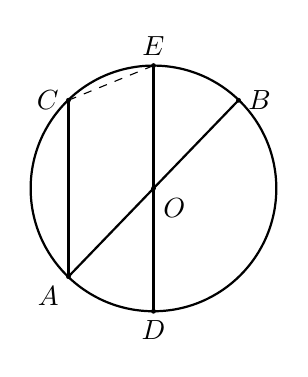
\begin{tikzpicture}[scale=0.8]
  \coordinate (O) at (0,0);
  \coordinate (A) at (-1.35,-1.4);
  \coordinate (B) at (1.35,1.4);
  \coordinate (E) at (0,1.95);
  \coordinate (D) at (0,-1.95);
  \coordinate (C) at (-1.35,1.4);
  \draw[thick] (O) circle (1.95);
  \draw[thick] (A)--(B);
  \draw[thick] (D)--(E);
  \draw[thick] (A)--(C);
  \draw[dashed] (C)--(E);
  \fill (O) circle (1.1pt) node[below right] {$O$};
  \fill (A) circle (1.1pt) node[below left] {$A$};
  \fill (B) circle (1.1pt) node[right] {$B$};
  \fill (C) circle (1.1pt) node[left] {$C$};
  \fill (D) circle (1.1pt) node[below] {$D$};
  \fill (E) circle (1.1pt) node[above] {$E$};
\end{tikzpicture}
\end{center}
\nopagebreak[4]
\end{question}
\begin{question}
\gkti{3}如果已知 $bx^2-4bx+2(a+c)=0$（$b\ne0$）有两个相等的实数根，求证：$a\text{、}b\text{、}c$ 成等差数列。

\Needspace{0.4\textheight}
\end{question}
\begin{question}
\gkti{4}

（1） 如图，为求河对岸某建筑物的高 $AB$，在地面上引一条基线 $CD=a$，测得 $\angle ACB=\alpha$，$\angle BCD=\beta$，$\angle BDC=\gamma$，求 $AB$。
\nopagebreak[4]
\begin{center}% 1977 年天津卷第 4(1) 题：河对岸建筑物高度测量
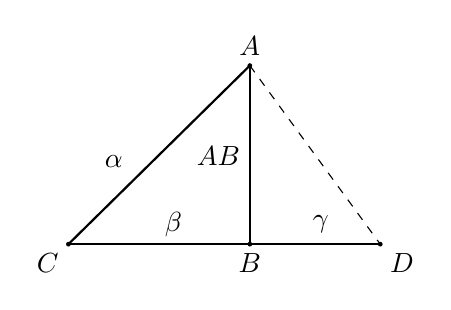
\begin{tikzpicture}[scale=0.72,>=stealth]
  \coordinate (B) at (0.7,0.1);
  \coordinate (A) at (0.7,3.25);
  \coordinate (C) at (-2.5,0.1);
  \coordinate (D) at (3.0,0.1);
  \draw[thick] (A)--(B);
  \draw[thick] (C)--(D);
  \draw[thick] (C)--(A);
  \draw[thick] (C)--(B);
  \draw[thick] (D)--(B);
  \draw[dashed] (A)--(D);
  \fill (A) circle (1.2pt) node[above] {$A$};
  \fill (B) circle (1.2pt) node[below] {$B$};
  \fill (C) circle (1.2pt) node[below left] {$C$};
  \fill (D) circle (1.2pt) node[below right] {$D$};
  \node at (-1.7,1.55) {$\alpha$};
  \node at (-0.65,0.45) {$\beta$};
  \node at (1.95,0.45) {$\gamma$};
  \node[left] at (0.7,1.65) {$AB$};
\end{tikzpicture}
\end{center}
\nopagebreak[4]
（2） 如果 $\alpha=30^\circ$，$\beta=75^\circ$，$\gamma=45^\circ$，$a=33$ 米，求建筑物 $AB$ 的高。（保留一位小数）

\end{question}
\begin{question}
\gkti{5}

（1） 求直线 $3x-2y+1=0$ 和 $x+3y+4=0$ 的交点坐标。

（2） 求通过上述交点，并同直线 $x+3y+4=0$ 垂直的直线方程。

\begin{gktip}
\Needspace{0.25\textheight}
\textbf{附加题}
\end{gktip}

\Needspace{5\baselineskip}
\textbf{附加题 6．} 求

\nopagebreak[4]
\[
\lim_{x\to0}\frac{\mathrm e^x-\mathrm e^{-x}-2x}{x-\sin nx}
\]

的值。

\Needspace{5\baselineskip}
\textbf{附加题 7．} 计算：

\nopagebreak[4]
\[
\int_0^4\frac{x+2}{\sqrt{2x+1}}\,\mathrm dx.
\]

\end{question}